\chapter{Annontated Examples}
\section{Preliminaries}

This chapter demonstrates the core functionality of the code. In Section \ref{sec:mansol}, we present steps necessary for running a manufactured solution problem.

In this section, we will go through several example problems for running \pkg{dgswem-v2}. In order to provide succint instructions to the reader, we introduce the following environment variables. We will assume that the following environment variables have been defined in the users environment:
\begin{lstlisting}{language=bash}
export DGSWEMV2_REPO=<path/to/dgswemv2_repo>
export DGSWEMV2_BUILD=<path/to/dgswemv2_build>
export DGSWEMV2_EXAMPLES=${DGSWEMV_REPO}/examples
\end{lstlisting}

Additionally, to keep the compile time of the application short, the cmake configuration does not automatically build the examples. To build the following examples, you will need to rerun your \pkg{cmake} build command with the additional option \lstinline{-DBUILD_EXAMPLES=On}.



\section{Manufactured Solution}
\label{sec:mansol}
The method of manufactured solutions presents an easy means of determining whether the solution is converging at the rates stipulated by the theoretical error estimates. In addition, since we obtain exact error estimates, the method of manufactured solutions may also be used to determine, whether or not errors have been introduced between parallel and serial implementations.

To avoid the stability-related difficulties associated with greatly varying mesh refinements, we evaluate the manufactured solution from~\cite{Wiraset2014}. For the manufactured solution, we set the solution to be equal to
\begin{align}
\zeta(x,y,t) &= 2 \zeta_0 \frac{ \cos \left( \omega(x - x_1) \right) \cos \left( \omega(y - y_1)\right) \cos(\omega t)}{
\cos \left( \omega(x_2 - x_1)\left) \cos \right( \omega(y_2 - y_1)\right)} \nonumber \\
q_x(x,y,t) &= \zeta_0 \frac{ \sin \left(\omega(x - x_1)\right) \cos\left(\omega(y - y_1)\right) \sin(\omega t)}{\cos\left( \omega ( x_2 - x_1)\right) \cos\left(\omega ( y_2 - y_1)\right)} \nonumber \\
q_y(x,y,t) &= \zeta_0 \frac{ \cos\left(\omega (x - x_1)\right) \sin\left( \omega(y -y_1)\right) \sin( \omega t)}{\cos \left( \omega ( x_ 2 - x_1)\right) \cos\left( \omega(y_2 - y_1)\right)} \nonumber
\end{align}
where $x_1 = 40,000\,\mathrm{m},\, x_2= 83,200\,\mathrm{m},\, y_1 = 10,000\,\mathrm{m},\,y_2 = 53,200\,\mathrm{m},\,\zeta_0 = 0.25\,\mathrm{m},\, \omega = 2 \pi/43,200\, \mathrm{rad}/\mathrm{s}$. Additionally, $g=9.81\,\mathrm{m}/\mathrm{s}^2$, and the bathymetry is constant with depth $H_0=2\,\mathrm{m}$. The source term is then obtained by applying the left hand side of the shallow water equations to the target solution.

The manufactured solutions can be run via the three following targets, which can be made as follows:
\begin{lstlisting}[language=bash]
cd ${DGSWEMV2_BUILD}
make MANUFACTURED_SOLUTION_SERIAL
make MANUFACTURED_SOLUTION_HPX
make MANUFACTURED_SOLUTION_OMPI
\end{lstlisting}
Note that for the HPX and the OMPI manufactured targets, the project must have the \lstinline{-DUSE_HPX} and \lstinline{-DUSE_OMPI} options set to \lstinline{On}, respectively.

The workflow for building the manufactured solution consists of three parts: (1) generating a mesh, (2) if necessary, partitioning the mesh, (3) running the simulation, and (4) interpreting the output.

\subsection{Generating the mesh}
For the generation of meshes, we use a \lstinline{yaml}-formatted input file. We have included an input file in
\begin{lstlisting}
${DGSWEMV2_EXAMPLES}/manufactured_solution/input_files/mesh_generator_input.yml
\end{lstlisting}
We have provided comments for the individual variables in the yaml files. One key aspect for improving the accuracy of the solution is the mesh resolution. To modulate these, \lstinline{num_x_subdivisions} and \lstinline{num_y_subdivisions} allows one to refine or coarsen the mesh appropriately. However, for now we leave them at their defaults. To generate the mesh, run the following commands
\begin{lstlisting}[language=bash]
cd ${DGSWEMV2_EXAMPLES}/manufactured_solution/input_files/
${DGSWEMV2_BUILD}/mesh_generators/rectangular_mesh_generator \
    mesh_generator_input.yml
\end{lstlisting}
This will generate a \lstinline{rectangular_mesh.14} file in the current directory. This is an ADCIRC-formatted meshfile.

\subsection{Partitioning the mesh (optional)}
Note that this section is only necessary if you are attempting to run the simulation in a distributed manner, i.e. using the OMPI or HPX executable. If you are only trying to run the simulation in serial, skip to the next subsection.

In order to run the simulation in parallel, the mesh must be broken into smaller pieces, which can then be assigned to individual processors. Since there exist stark contrasts in the send latencies between two processors on the same node versus processors that might be connected via an interconnect, we require the user to specify the number of localities (i.e. private memory address spaces) in addition to the number of partitions to allow for the mesh partitioner to optimize these interconnect effects.

The partitioner executable can be found in
\begin{lstlisting}[language=bash]
${DGSWEMV2_BUILD}/partitioner/partitioner
\end{lstlisting}
and running the executable without any arguments will provide usage information. In particular, the variables mean the following:
\begin{itemize}
\item \lstinline{<input filename>}: The name of the input file used to run the execution.
\item \lstinline{<number of partitions>}: The number of partitions the mesh is to be partitioned into.
\item \lstinline{<number of nodes>}: The number of hardware localities the simulation is to be run on.
\item \lstinline{<ranks per locality>}: The number of ranks per locality. 
\item \lstinline{<rank balanced>}: Whether or not the constraints should be balanced across the individual submeshes. Note that the entry options are \lstinline{true} or \lstinline{false}. Recommended for OpenMP/MPI.
\end{itemize}
Our two parallelization strategies rely on different parallel execution models. Thus the inputs for either version need to be slightly modified. In the following two subsections we outline, the differences in general, but also provide concrete numbers to allow the user to proceed.
\subsubsection{Partitioning for HPX}
The HPX execution model varies from that of traditional parallelization strategies in that the number of partitions does not correspond to any hardware concept. For example, traditional MPI implementations assigned one rank per core, and insofar the number of partitions equalled the number of cores. For HPX, the number of partitions is roughly proportional to the number of tasks executed on that locality. \emph{Oversubscribing} meshes --- assigning more meshes to the locality than there are cores --- can lead to desirable behavior in the form of hiding of send latencies. However, the user needs to be careful to avoid exposing too fine grain parallelism in the form of too many meshes, because task overhead will dominate the execution time and lead performance degradation.

To continue the example for an HPX parallelization, we recommend running:
\begin{lstlisting}[language=bash]
cd ${DGSWEMV2_EXAMPLES}/manufactured_solution/input_files
${DGSWEMV2_BUILD}/partitioner/partitioner\
    dgswemv2_input.15 4 1
\end{lstlisting}
This should generate, 4 \lstinline{meta}-formatted mesh files. The \lstinline{meta}-format isn't an official mesh format, but rather a simple method of representing the mesh internally for the \pkg{dgswem-v2} application, and 4 \lstinline{dbmd}-formatted files, which encapsulate the distributed metadata information required to ensure that submeshes appropriately communication with one another. In addition, we will have generated an updated input file specifically for running parallel meshes. For this example, it's 
\lstinline{dgswemv2_input_parallelized.15}.

\subsubsection{Partitioning for OpenMP/MPI}
Partitioning for the MPI+OpenMP implementation is slightly, different. Ratio of number of partitions to number of threads should correspond to the number of threads available on each node. However, it's also possible to run a flat MPI implementation by modifying the \lstinline{<ranks per locality>} option. This option will correspond to the number MPI ranks on each node.

Additionally, since submeshes are mapped statically to threads, we recommend setting the \lstinline{<rank balanced>} option to \lstinline{true}. For applications with varying load across the elements, e.g. in the case of wetting and drying, we would like to balance load and memory constraints across the submeshes. Ultimately, the performance will be constrained along the critical path, for statically mapped parallelizations optimal performance is achieved when each submesh roughly has the same amount of work. Note that this is not necessary for the HPX parallelization, which implements aggressive on-node work stealing.

To generate a mesh partitioning for this parallelization, we run
\begin{lstlisting}[language=bash]
cd ${DGSWEMV2_EXAMPLES}/manufactured_solution/input_files
${DGSWEMV2_BUILD}/partitioner/partitioner\
   dgswemv2_input.15 2 1 2 true
\end{lstlisting}
This configuration will result in a flat MPI run. With 2 MPI ranks. Note that similar to the HPX run, we generate both \lstinline{meta} mesh files and \lstinline{dbmd} connectivity information and an updated \lstinline{dgswemv2_input_paralllelized.15} input file.
\subsection{Running the simulation}
For each of the three execution modes --- serial, with HPX, and with MPI+OpenMP --- we have a separate executable.
To execute the serial implementation, run
\begin{lstlisting}[language=bash]
cd ${DGSWEMV2_EXAMPLES}/manufactured_solution/input_files
mkdir -p output
${DGSWEMV2_BUILD}/examples/MANUFACTURED_SOLUTION_SERIAL\
    dgswemv2_input.15
\end{lstlisting}
For the MPI and HPX versions, we assume that the parallel launcher, would be accessible through some \lstinline{<mpirun>} command, e.g. on a slurm based system this might \lstinline{srun}. The MPI-version can then be executed via
\begin{lstlisting}[language=bash]
cd ${DGSWEMV2_EXAMPLES}/manufactured_solution/input_files
mkdir -p ouptut
<mpirun> ${DGSWEMV2_BUILD}/examples/MANUFACTURED_SOLUTION_OMPI\
    dgswemv2_input.15
\end{lstlisting}
For the HPX version, the execution command depends on the set-up of the system. If there is no distributed aspect to your computing environment, you do not need a distributed launcher like \lstinline{srun}. Thus, for the reader running the simulation on their laptop, i.e. with one locality, the HPX example can be run as
\begin{lstlisting}[language=bash]
cd ${DGSWEMV2_EXAMPLES}/manufactured_solution/input_files
mkdir -p output
${DGSWEMV2_BUILD}/examples/MANUFACTURED_SOLUTION_HPX\
    dgswemv2_input.15
\end{lstlisting}

\subsection{Intepreting the Output}
\pkg{dgswem-v2} writes output in several forms. Firstly, in the \lstinline{output} folder that was created in the \texttt{\$\{DGSWEMV2\}\_EXAMPLES/manufactured\_solution} directory. You will find a log file name \lstinline{log} and \texttt{vtk}-formatted output. The output can be visualized using a package like \pkg{paraview}. A sample image of what the output should look like is shown in Figure \ref{fig:mansol}.
\begin{figure}
\centering
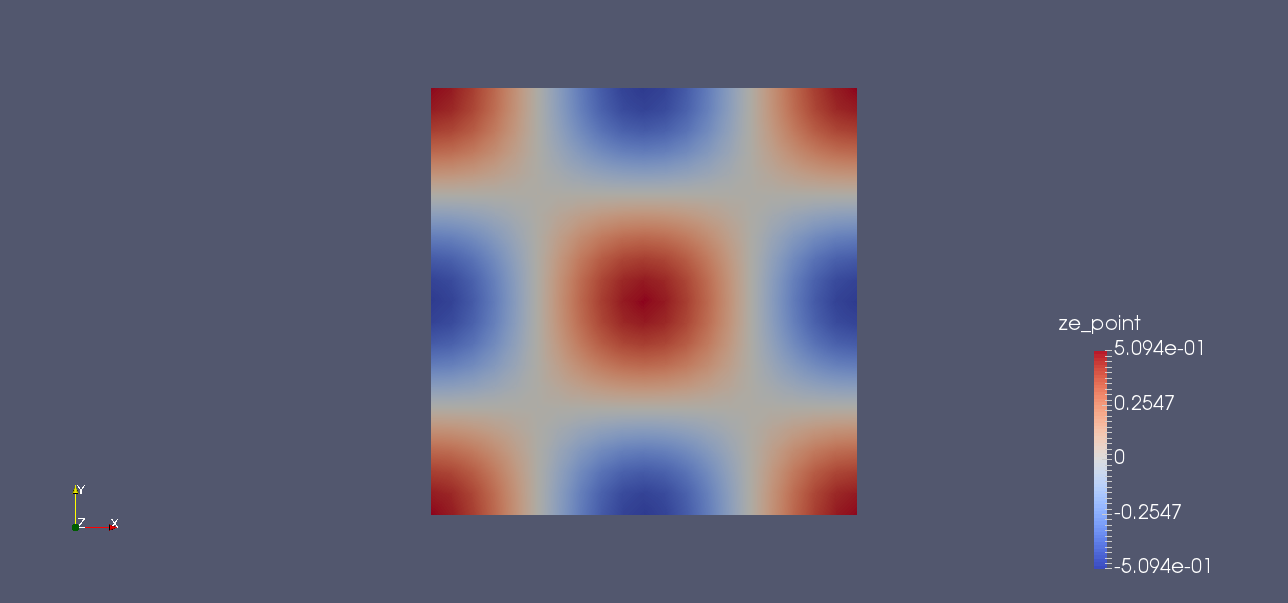
\includegraphics[width = 0.8 \textwidth]{{images/man_sol}.png}
\caption{Sample output of the manufactured solution output.}
\label{fig:mansol}
\end{figure}
\section{1D Inlet}
\label{sec:inlet}